\section{Dataset Description}

\iffalse
\subsection{\acrfull{kegg}}
\acrfull{kegg} is a community-driven database which contains large-scale molecular datasets generated by genome sequencing and high-throughput experimental techniuqe.\citep{Kanehisa2000, ozturk2018deepdta} We use \acrshort{kegg} DRUG dataset for finding the interaction set between DRUG and PROTEIN. The interaction score is :
\fi

\subsection{Kinase Inhibitor Bioactivity (KIBA)} \label{section:kiba}
The \acrfull{kiba} Scores are collected from the publicly made available dataset~\citep{Tang2013}. The scores are based on thermodynamic constants K\textsubscript{i} and K\textsubscript{d} and, remaining enzyme activity(Activity \% --  IC\textsubscript{50}).

% \begin{flushright}
\begin{equation}
  KIBA = \begin{cases}
    K_i . {adj} & \quad {if} \; {IC_{50}\: and\, K_i \,are\, present} \\
    K_b.{adj} & \quad {if}  {IC_{50} \, and \, K_d \, are \, present} \\
    \frac{K_i . {adj} \; K_b.{adj}}{2} & \quad {if\, IC_{50}\,,K_i\, and \,K_d\, are\, present}
  \end{cases}
   \label{eq:kiba}
\end{equation}
where,
\begin{equation}
K_i.{adj} = \frac{IC_{50}}{1 + L_i(IC_{50}/K_i)}
\label{eq:ki_adj}
\end{equation}

\begin{equation}
K_d.{adj} = \frac{IC_{50}}{1 + L_d(IC_{50}/K_d)}
\end{equation}
where L\textsubscript{d} and L\textsubscript{i} are parameters defining weights of IC\textsubscript{50} in model adjustments for K\textsubscript{i} and K\textsubscript{b} 
% \end{flushright}

For a kinase inhibitor drug−target interaction, we consider the medians of three major bioactivity types IC\textsubscript{50}, K\textsubscript{i}, K\textsubscript{d} where
IC\textsubscript{50} \citep{Tang2013} is the concentration at which the inhibitor causes a 50\% inhibition of enzymatic activity and K\textsubscript{i} is defined by \begin{equation}
    Ki = \frac{IC_{50}} {1 + [S]  K_m}
    \label{eq:ki}
\end{equation} 
where,  [{S}] is the experimental substrate concentration and K\textsubscript{m} is the concentration of the substrate.

\iffalse
\begin{equation}
    \tau= \frac{(a−b)}{n(n − 1)/2}   
    \label{eq:tau}
  \end{equation}
  { Here {a} and {b} represent the number of concordant pairs and discordant pairs respectively. }
\fi


All the bioactivity types are available from CHEMBL\citep{Gaulton2017}. Based on interaction data available, we remove the unknown values and obtained a total of \arabic{no_interactions} interaction KIBA score values in the range of -3.09 to 17.8. With the standard deviation of 1.22, it represents a total of \arabic{no_proteins} proteins and \arabic{no_drugs} drugs.

\begin{figure}
  \label{fig:interactions_summary}
  \centering
  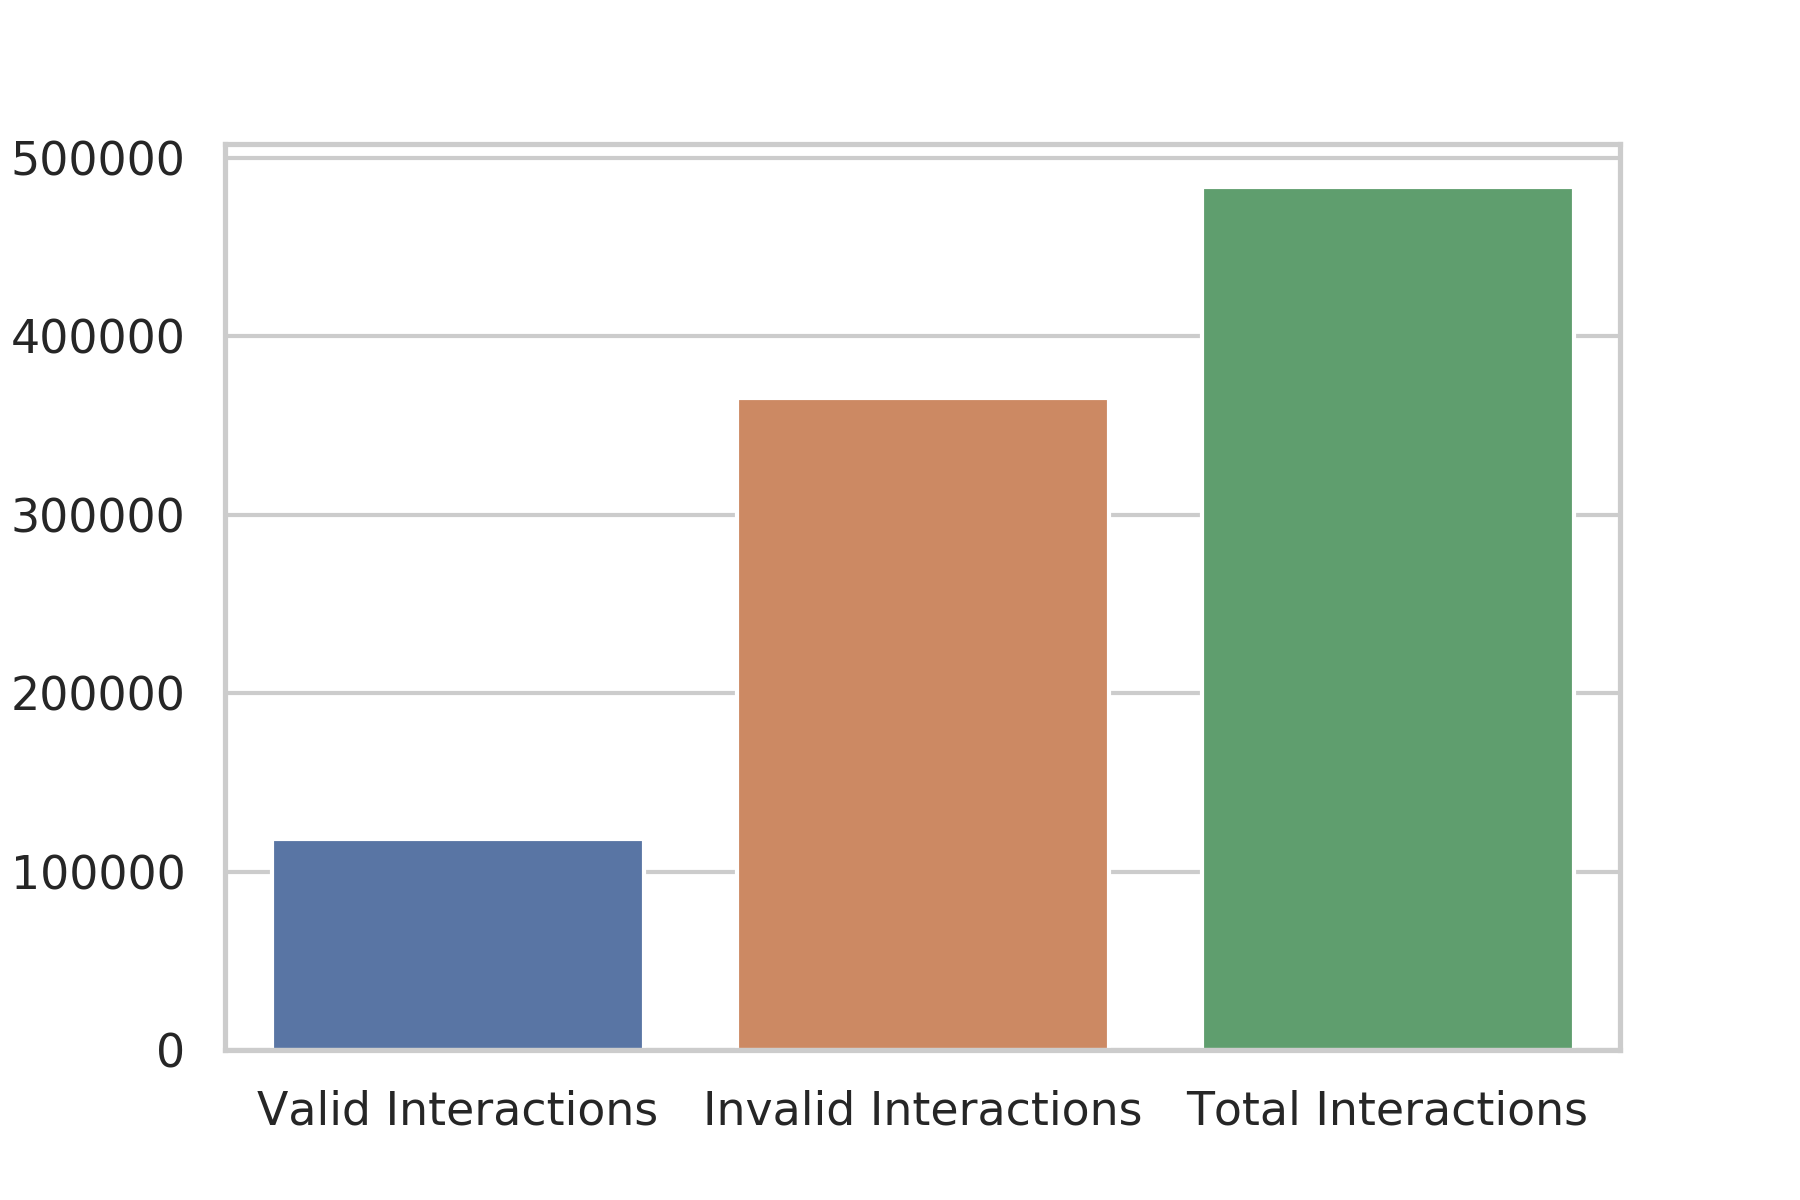
\includegraphics[width=.7\textwidth]{dataset/images/interactions_summary.png}
  \caption{Bar Chart of interactions available in dataset}
\end{figure}
